\documentclass[tikz,border=8pt]{standalone}
\usepackage[T1]{fontenc}
\usepackage{lmodern}
\usepackage{tikz}
\usetikzlibrary{arrows.meta,calc,decorations.pathreplacing,fit,matrix,positioning}

\definecolor{cornellred}{HTML}{B31B1B}
\definecolor{ink}{HTML}{202124}
\definecolor{muted}{HTML}{667085}
\definecolor{line}{HTML}{AEB8C6}
\definecolor{paper}{HTML}{FFFFFF}
\definecolor{soft}{HTML}{F5F7FA}
\definecolor{camera}{HTML}{E8F4FF}
\definecolor{memory}{HTML}{F0F7EC}
\definecolor{compute}{HTML}{FFF3E6}
\definecolor{display}{HTML}{F7ECF3}
\definecolor{verify}{HTML}{EFEAFE}

\tikzset{
  font=\sffamily,
  flow/.style={
    -{Latex[length=2.6mm,width=1.8mm]},
    draw=muted,
    line width=0.8pt,
    rounded corners=2pt
  },
  dataflow/.style={
    flow,
    draw=cornellred
  },
  block/.style={
    rectangle,
    rounded corners=3pt,
    draw=line,
    line width=0.8pt,
    fill=paper,
    align=center,
    minimum width=28mm,
    minimum height=10mm,
    inner xsep=4pt,
    inner ysep=4pt
  },
  smallblock/.style={
    block,
    minimum width=22mm,
    minimum height=8mm,
    font=\sffamily\scriptsize
  },
  title/.style={
    font=\sffamily\bfseries\large,
    text=ink
  },
  labeltext/.style={
    font=\sffamily\scriptsize,
    text=muted,
    align=center
  },
  camera_block/.style={block, fill=camera, draw=blue!45!black},
  memory_block/.style={block, fill=memory, draw=green!45!black},
  compute_block/.style={block, fill=compute, draw=orange!65!black},
  display_block/.style={block, fill=display, draw=purple!45!black},
  verify_block/.style={block, fill=verify, draw=violet!50!black},
  groupbox/.style={
    draw=line,
    rounded corners=5pt,
    line width=0.7pt,
    fill=soft,
    inner sep=7pt
  }
}


\begin{document}
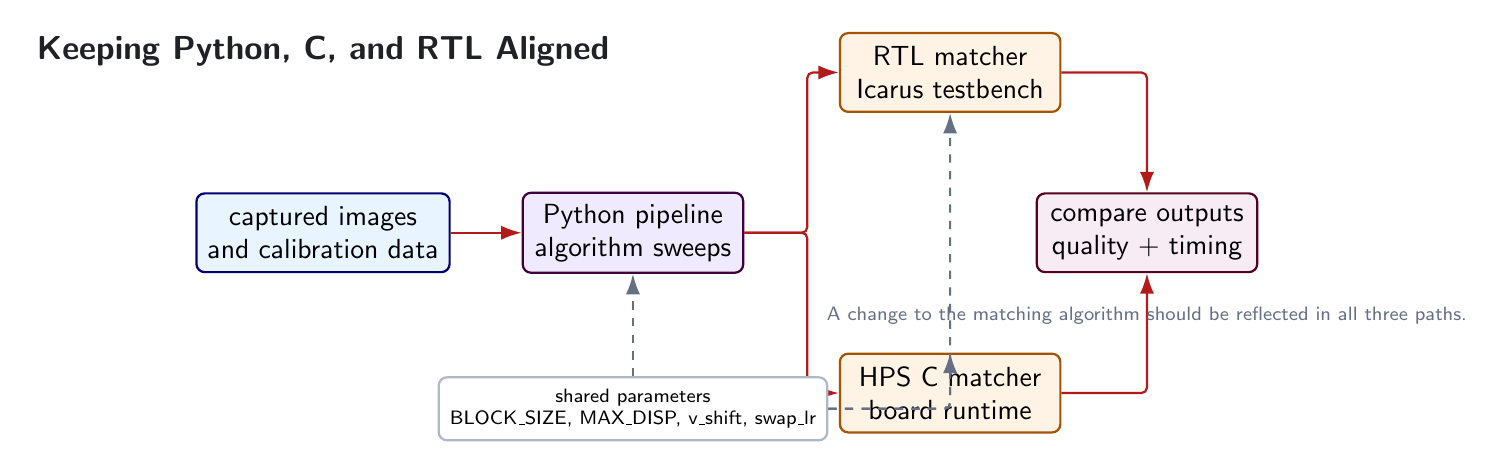
\begin{tikzpicture}[node distance=8mm and 9mm]
  \node[title] at (0, 2.3) {Keeping Python, C, and RTL Aligned};

  \node[camera_block] (fixtures) {captured images\\and calibration data};
  \node[verify_block, right=of fixtures] (python) {Python pipeline\\algorithm sweeps};
  \node[compute_block, above right=10mm and 12mm of python] (rtl) {RTL matcher\\Icarus testbench};
  \node[compute_block, below right=10mm and 12mm of python] (cmodel) {HPS C matcher\\board runtime};
  \node[display_block, right=37mm of python] (compare) {compare outputs\\quality + timing};

  \draw[dataflow] (fixtures) -- (python);
  \draw[dataflow] (python.east) -- ++(8mm,0) |- (rtl.west);
  \draw[dataflow] (python.east) -- ++(8mm,0) |- (cmodel.west);
  \draw[dataflow] (rtl.east) -| (compare.north);
  \draw[dataflow] (cmodel.east) -| (compare.south);

  \node[smallblock, fill=paper, below=13mm of python, minimum width=47mm] (params) {shared parameters\\BLOCK\_SIZE, MAX\_DISP, v\_shift, swap\_lr};
  \draw[flow, dashed] (params.north) -- (python.south);
  \draw[flow, dashed] (params.east) -| (rtl.south);
  \draw[flow, dashed] (params.east) -| (cmodel.north);

  \node[labeltext, below=3mm of compare] {A change to the matching algorithm should be reflected in all three paths.};
\end{tikzpicture}
\end{document}

